\subsection{Appearance of new words}

We consider the rate at which new 1-grams are incorporated in the vocabulary, and the nature of those words,  as a crucial component of linguistic drifts. It was thus important to come up with a reliable way to quantify this process .\\

A simple approach to estimate the apparition of new words would be to sum up the number of distinct 1-grams for each year and then monitor its evolution. But this suffers several drawbacks : first the remaining OCR errors, that still account for a substantial portion of the distinct 1-grams,  would be incorrectly considered as emerging words.  Furthermore, it would not provide any clue about the actual amount of words entering/exiting the set of used words, but only snapshots of how many words are in fashion at any point in time. Those two aspects would in our opinion have strongly distorted the resulting figures, this is why we opted for a different procedure.\\

TODO \\

\begin{figure}[h!]
        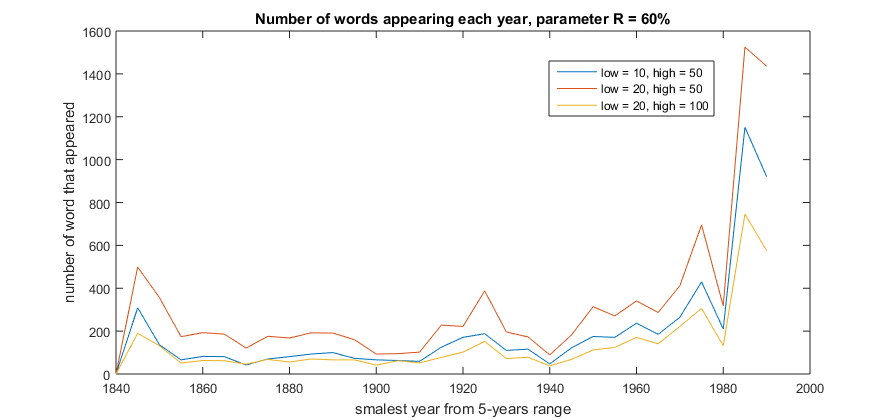
\includegraphics[scale=0.65]{Pictures/statistics/appearing-words/word-appearing-ratio60.png}
        \caption{New words detection with tolerance rate R = 60\%}
        \label{ratio60}
\end{figure}
\begin{figure}[h!]
        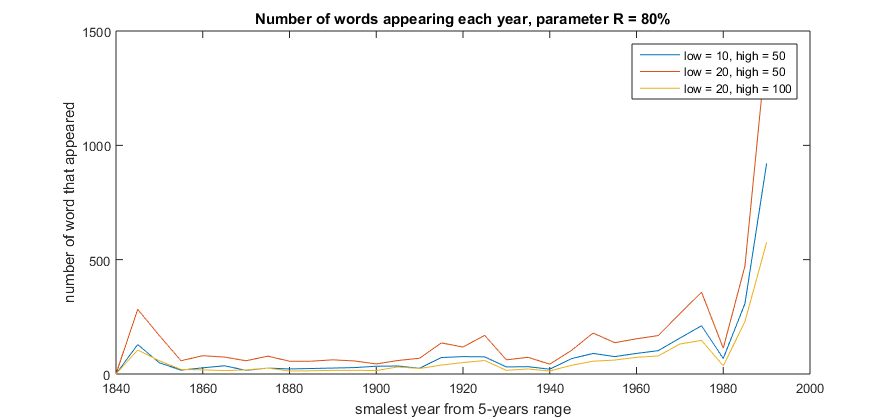
\includegraphics[scale=0.65]{Pictures/statistics/appearing-words/word-appearing-ratio80.png}
        \caption{New words detection with tolerance rate R = 80\%}
        \label{ratio80}
\end{figure}